\documentclass[10pt]{beamer}

\usepackage{hyperref}
\hypersetup{
    colorlinks=true,
    linkcolor=black,
    filecolor=black,
    urlcolor=blue,
    citecolor=black
}

\usetheme[progressbar=foot]{metropolis}
\usepackage{appendixnumberbeamer}

\usepackage{booktabs}
\usepackage[scale=2]{ccicons}

\usepackage{pgfplots}
\usepgfplotslibrary{dateplot}

\usepackage{xspace}
\usepackage{xcolor}

\DeclareMathOperator{\stdev}{stdev}
\DeclareMathOperator{\var}{var}
\DeclareMathOperator{\cov}{cov}
\DeclareMathOperator{\corr}{corr}
\DeclareMathOperator{\prob}{prob}
\DeclareMathOperator{\n}{n}
\DeclareMathOperator{\N}{N}
\DeclareMathOperator{\Cov}{Cov}

\newcommand{\D}{\mathrm{d}}
\newcommand{\E}{\mathrm{e}}
\newcommand{\mye}{\ensuremath{\mathsf{E}}}
\newcommand{\myreal}{\ensuremath{\mathbb{R}}}

\setbeamertemplate{frame footer}{MGMT 675}


\setbeamertemplate{title page}{
  \begin{centering}
    \begin{beamercolorbox}[sep=8pt,center]{title}
      \usebeamerfont{title}\inserttitle\par%
      \ifx\insertsubtitle\@empty%
      \else%
        \vskip0.25em%
        {\usebeamerfont{subtitle}\usebeamercolor[fg]{subtitle}\insertsubtitle\par}%
      \fi%     
    \end{beamercolorbox}%
    \vfill
    \begin{beamercolorbox}[sep=8pt,center]{date}
      \usebeamerfont{date}\insertdate
    \end{beamercolorbox}
    \vskip0.5em
    {\usebeamercolor[fg]{titlegraphic}\inserttitlegraphic\par}
  \end{centering}
}

\title{Data Visualization}
\subtitle{MGMT 675: AI-Assisted Financial Analysis}
\titlegraphic{
\includegraphics[height=1cm]{../docs/RiceBusiness-transparent-logo-sm.png}}
\date{}
\begin{document}

\begin{frame}[plain]
\titlepage
\end{frame}

\begin{frame}{Outline}
\begin{itemize}
\item Illustrate AI + python visualization by an example: try to understand PE ratios
\begin{itemize}
\item How they depend on financial ratios and growth rates
\item How the dependence may vary by sector and size 
\end{itemize}
\item Next week: prediction by neural networks
\end{itemize}
\end{frame}

\section{Data}

\begin{frame}{financials.xlsx}
\begin{itemize}
\item Download financials.xlsx from the schedule page.
\item Filtered to net income > 0. 1300+ firms
\item PE = price / EPS.  Price is closing price on 4/7/2025.  EPS is most recent annual. 
\item Various financial ratios from most recent annual report and some one-year growth rates 
\item Other categorical and continuous variables
\end{itemize}
\end{frame}

\begin{frame}{Ratios and Growth Rates}
\begin{itemize}
  \item DuPont factors:
  \begin{itemize}
    \item lvg = assets / equity
 \item assetturnover = revenue / assets
 \item grossmargin = gross profit / revenue
 \item netinc\_grprof = net income / gross profit
  \end{itemize}
  \item Other ratios:
  \begin{itemize}
\item roe, roa, netmargin = net income / (equity, assets, or revenue)
\item ebitmargin, ebitdamargin = (EBIT or EBITDA) / revenue
\item de = liabilities / equity
\item currentratio = current assets / current liabilities
\item payoutratio = dividends / net income
\end{itemize}
\item Growth rates: eps\_gr, asset\_gr, revenue\_gr = eps, assets, or revenue growth
\end{itemize}
\end{frame}

\begin{frame}{Other Categorical and Continuous Variables}
\begin{itemize}
\item Categorical: sector, scalerevenue
\item Continuous: assets, equity, revenue
\item Can create our own categories from continuous variables 
\end{itemize}
\end{frame}

\begin{frame}{Filtering}
  \begin{itemize}
    \item The data has already been filtered to EPS $>$ 0
    \item PE is heavily right-skewed.  You will probably want to ask Julius to filter the right tail, e.g., PE $<$ 100.
    \item You may also want to filter to subsets of sector and scalerevenue
    \item We can create your own categorical variables.  E.g., ask Julius to create a variable equal to the leverage quintile.
  \end{itemize}
\end{frame}

\section{Plots}

\begin{frame}{Plot Features You can Control}
  \begin{itemize}
    \item Font sizes
    \item Background color
    \item Color templates
    \item Gridlines or not 
    \item Legend or not and where to locate it
    \item Figure title and axis labels
    \item Multiple plots in a figure (e.g, 2x2 layout)
    \item Annotate points with text and arrows
    \item Add regression lines
    \item Really, anything you can think of.
  \end{itemize}
\end{frame}

\begin{frame}{Output Types}
\begin{itemize}
\item jpeg, png, pdf
\item Word doc or PowerPoint deck
\item interactive html
\end{itemize}
\end{frame}

\section{Examples}



\begin{frame}[plain]
  \begin{center}
  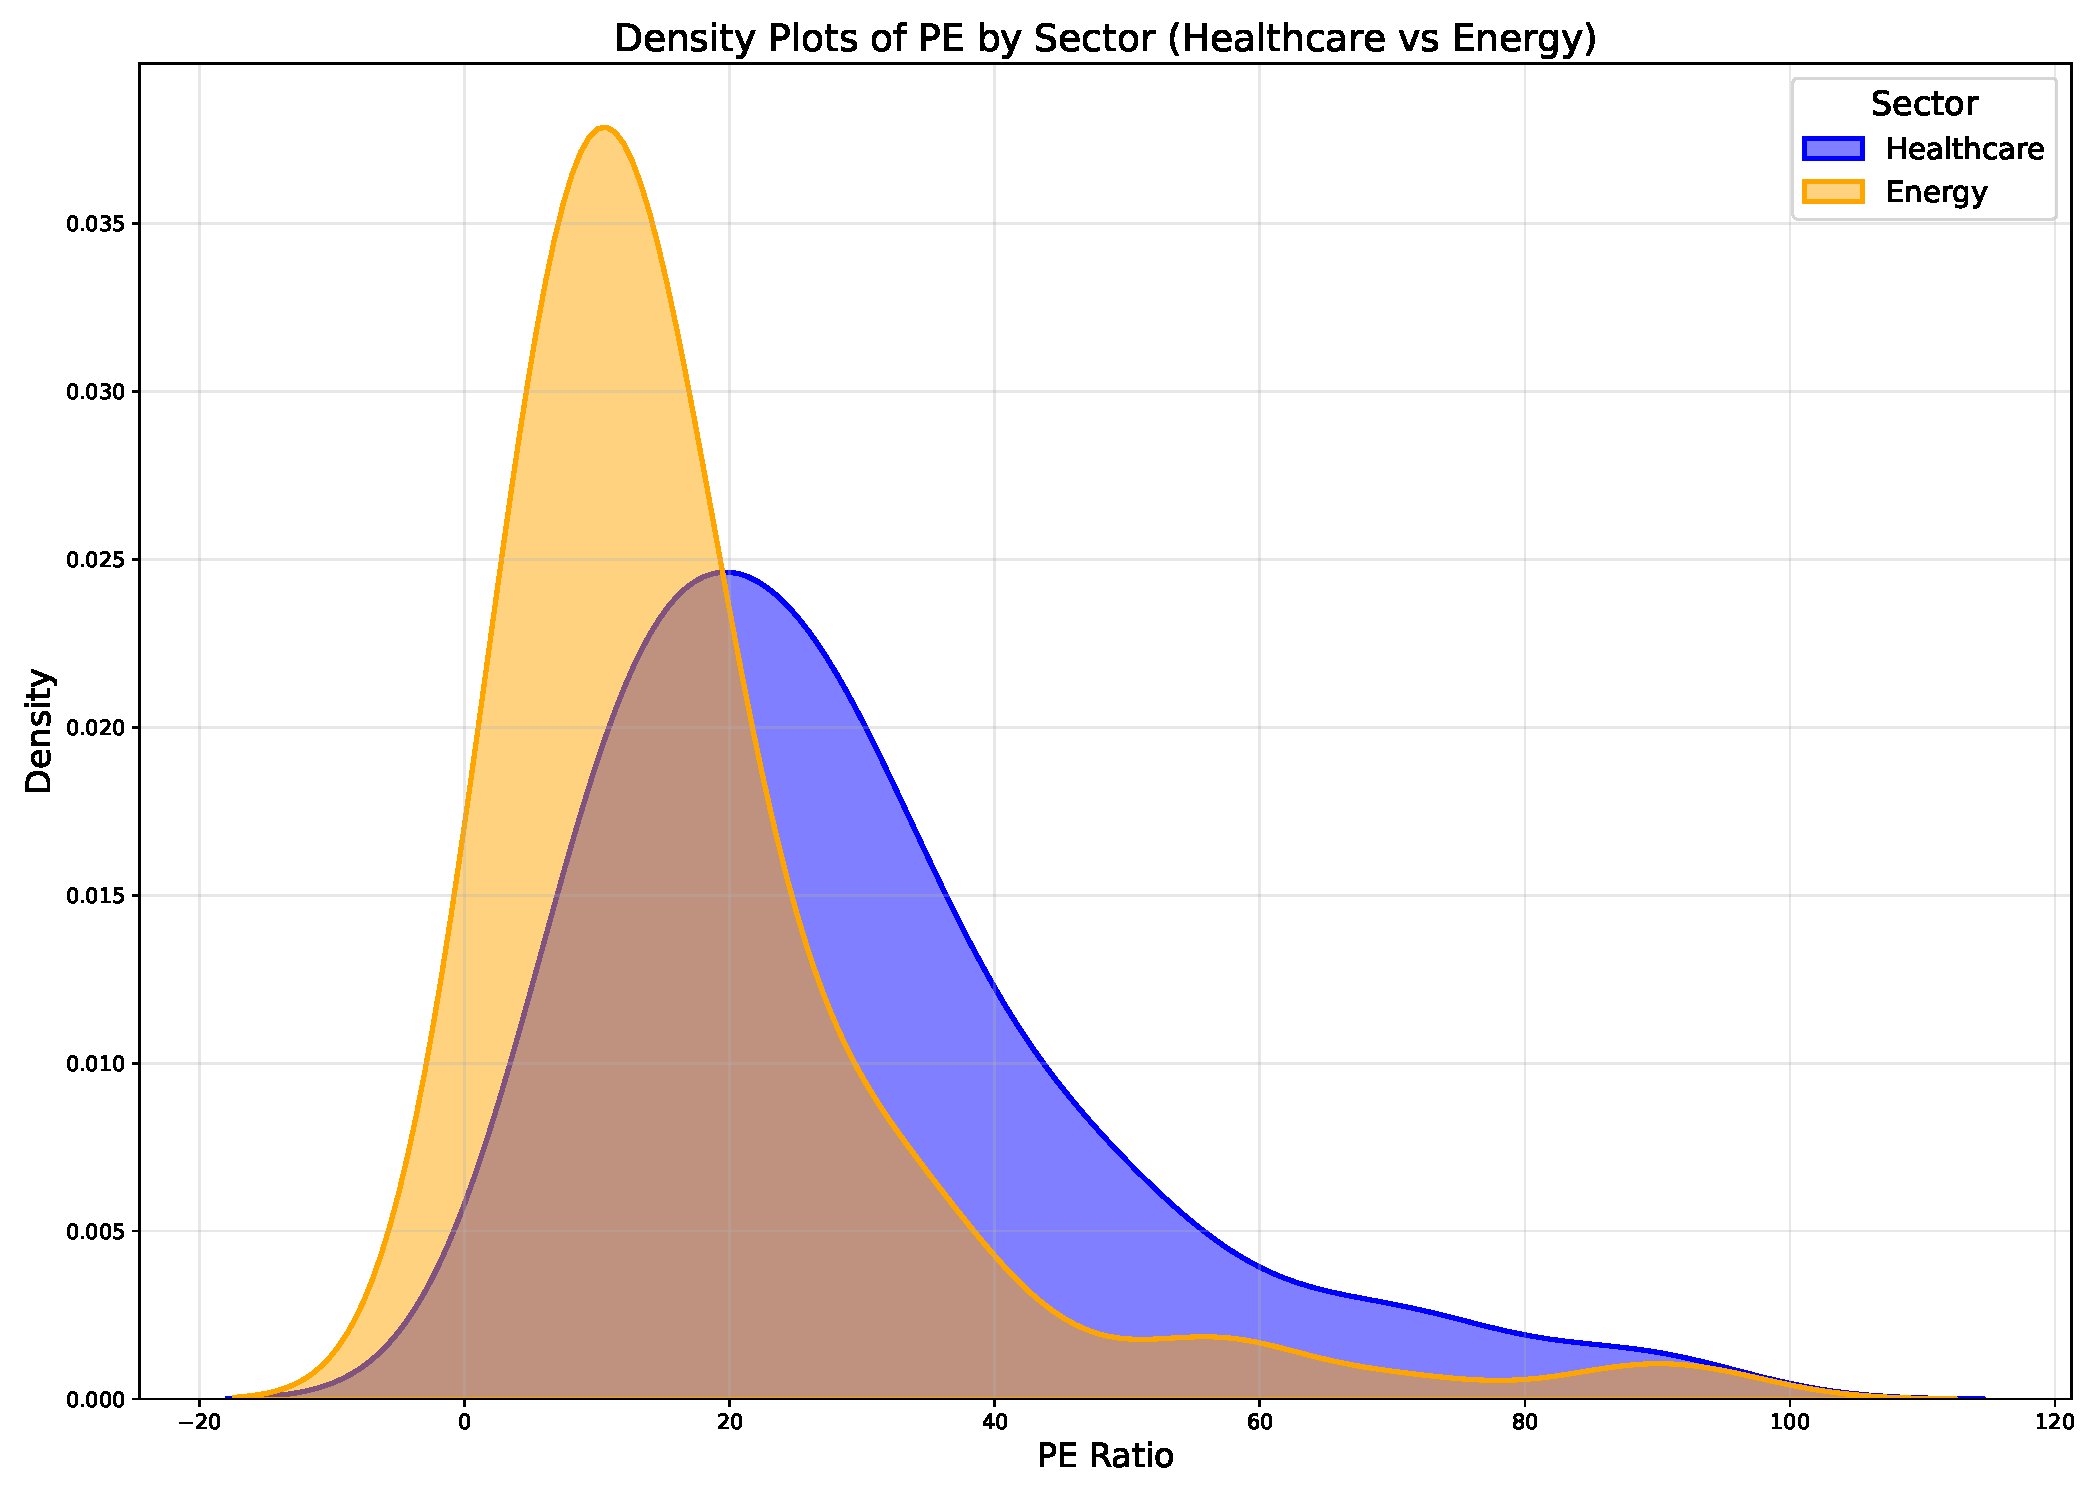
\includegraphics[width=0.9\textwidth]{financial_images/density_plot_pe_updated.pdf}
  \end{center}
\end{frame}

\begin{frame}[plain] 
  \begin{center}
  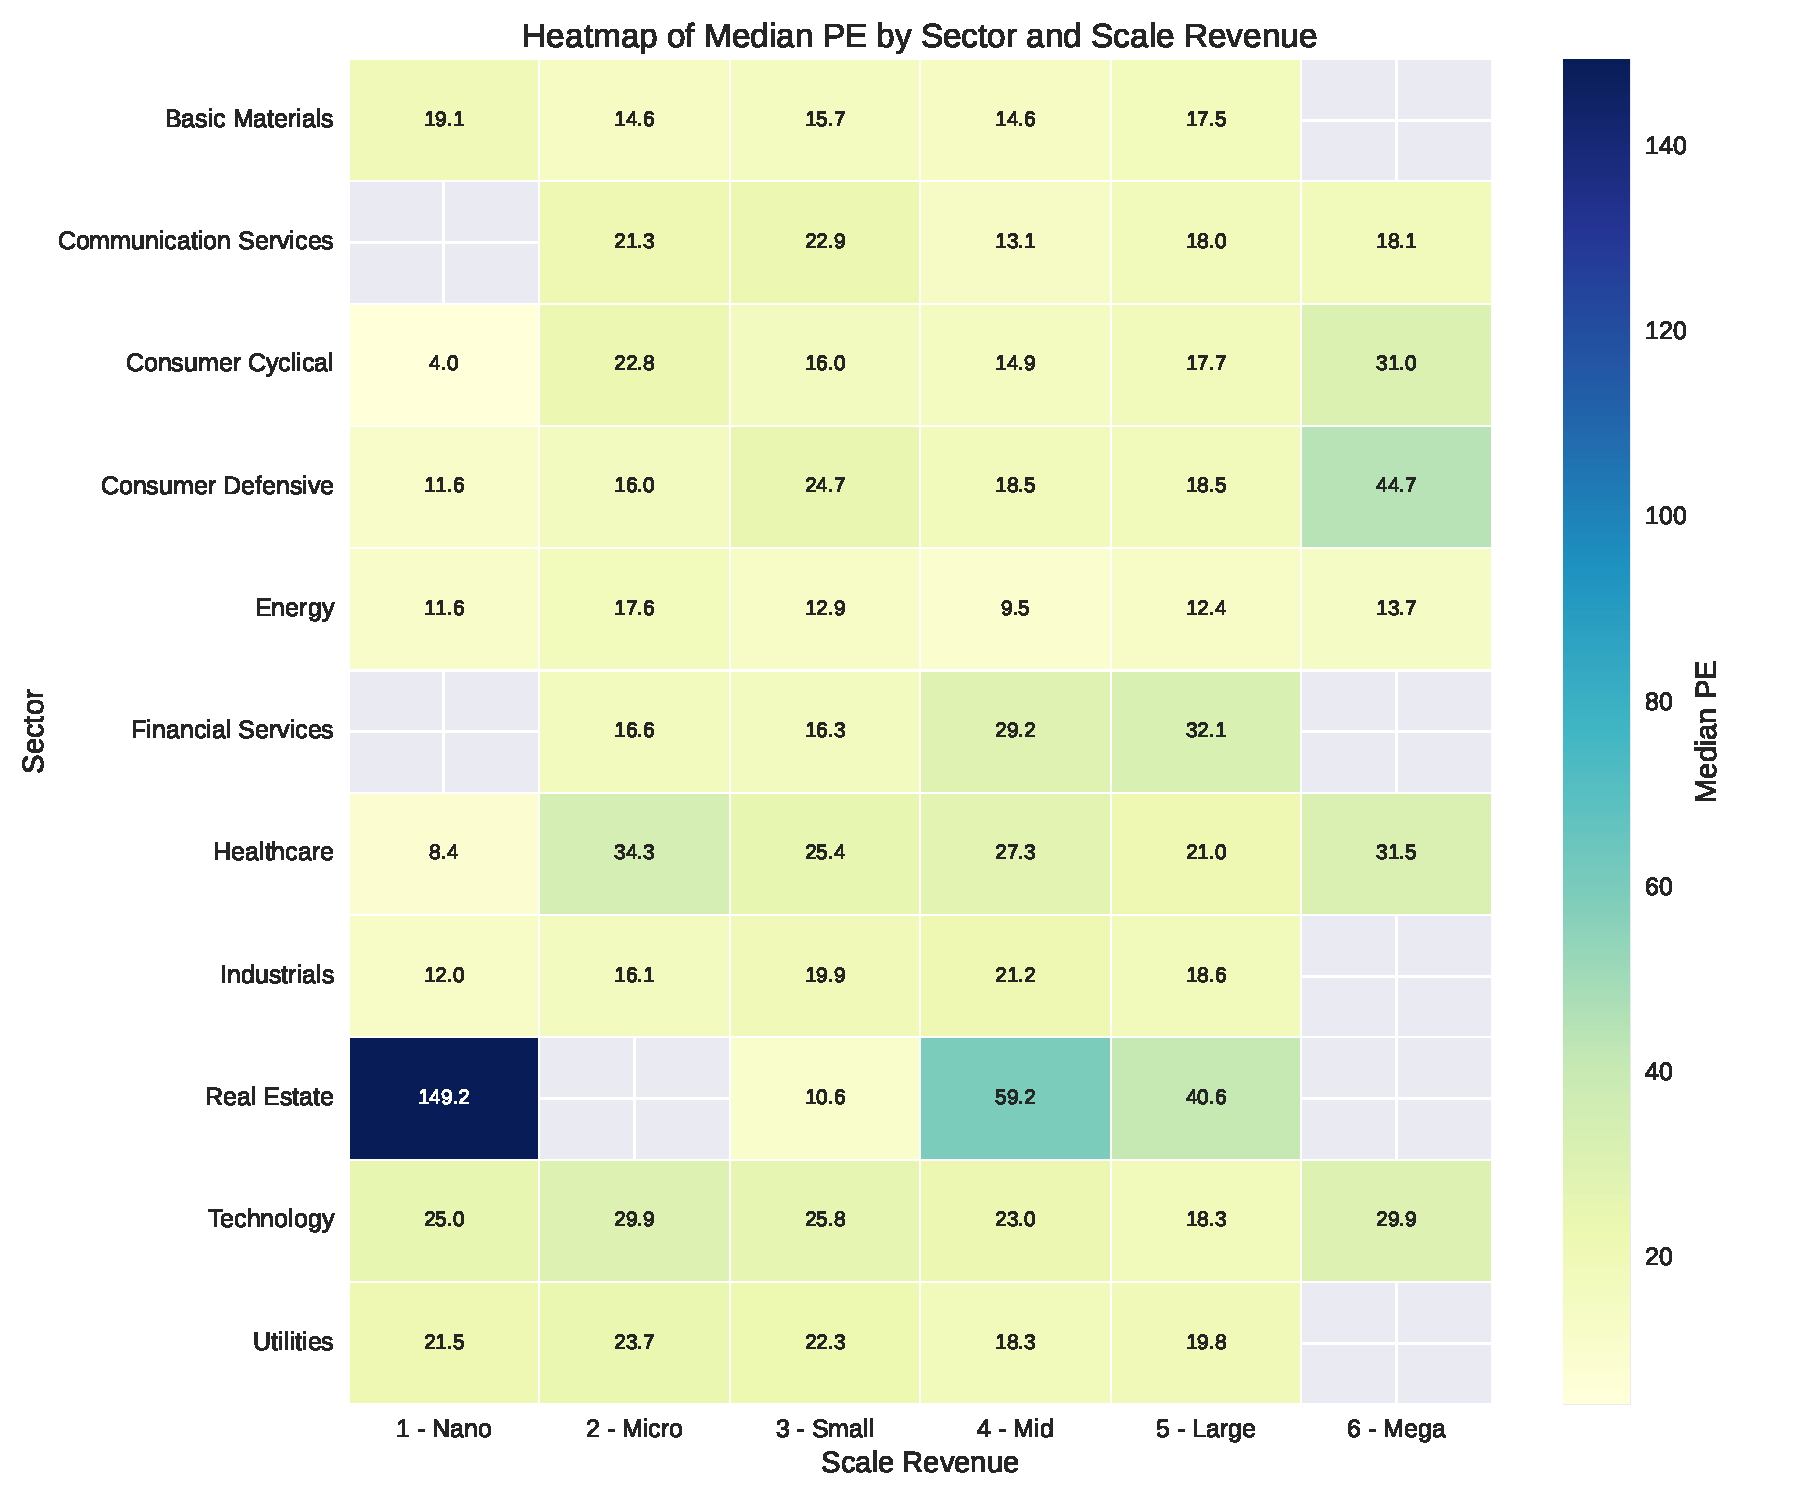
\includegraphics[width=0.9\textwidth]{financial_images/heatmap_pe.pdf}
  \end{center}
\end{frame}


\begin{frame}[plain]
  \begin{center}
  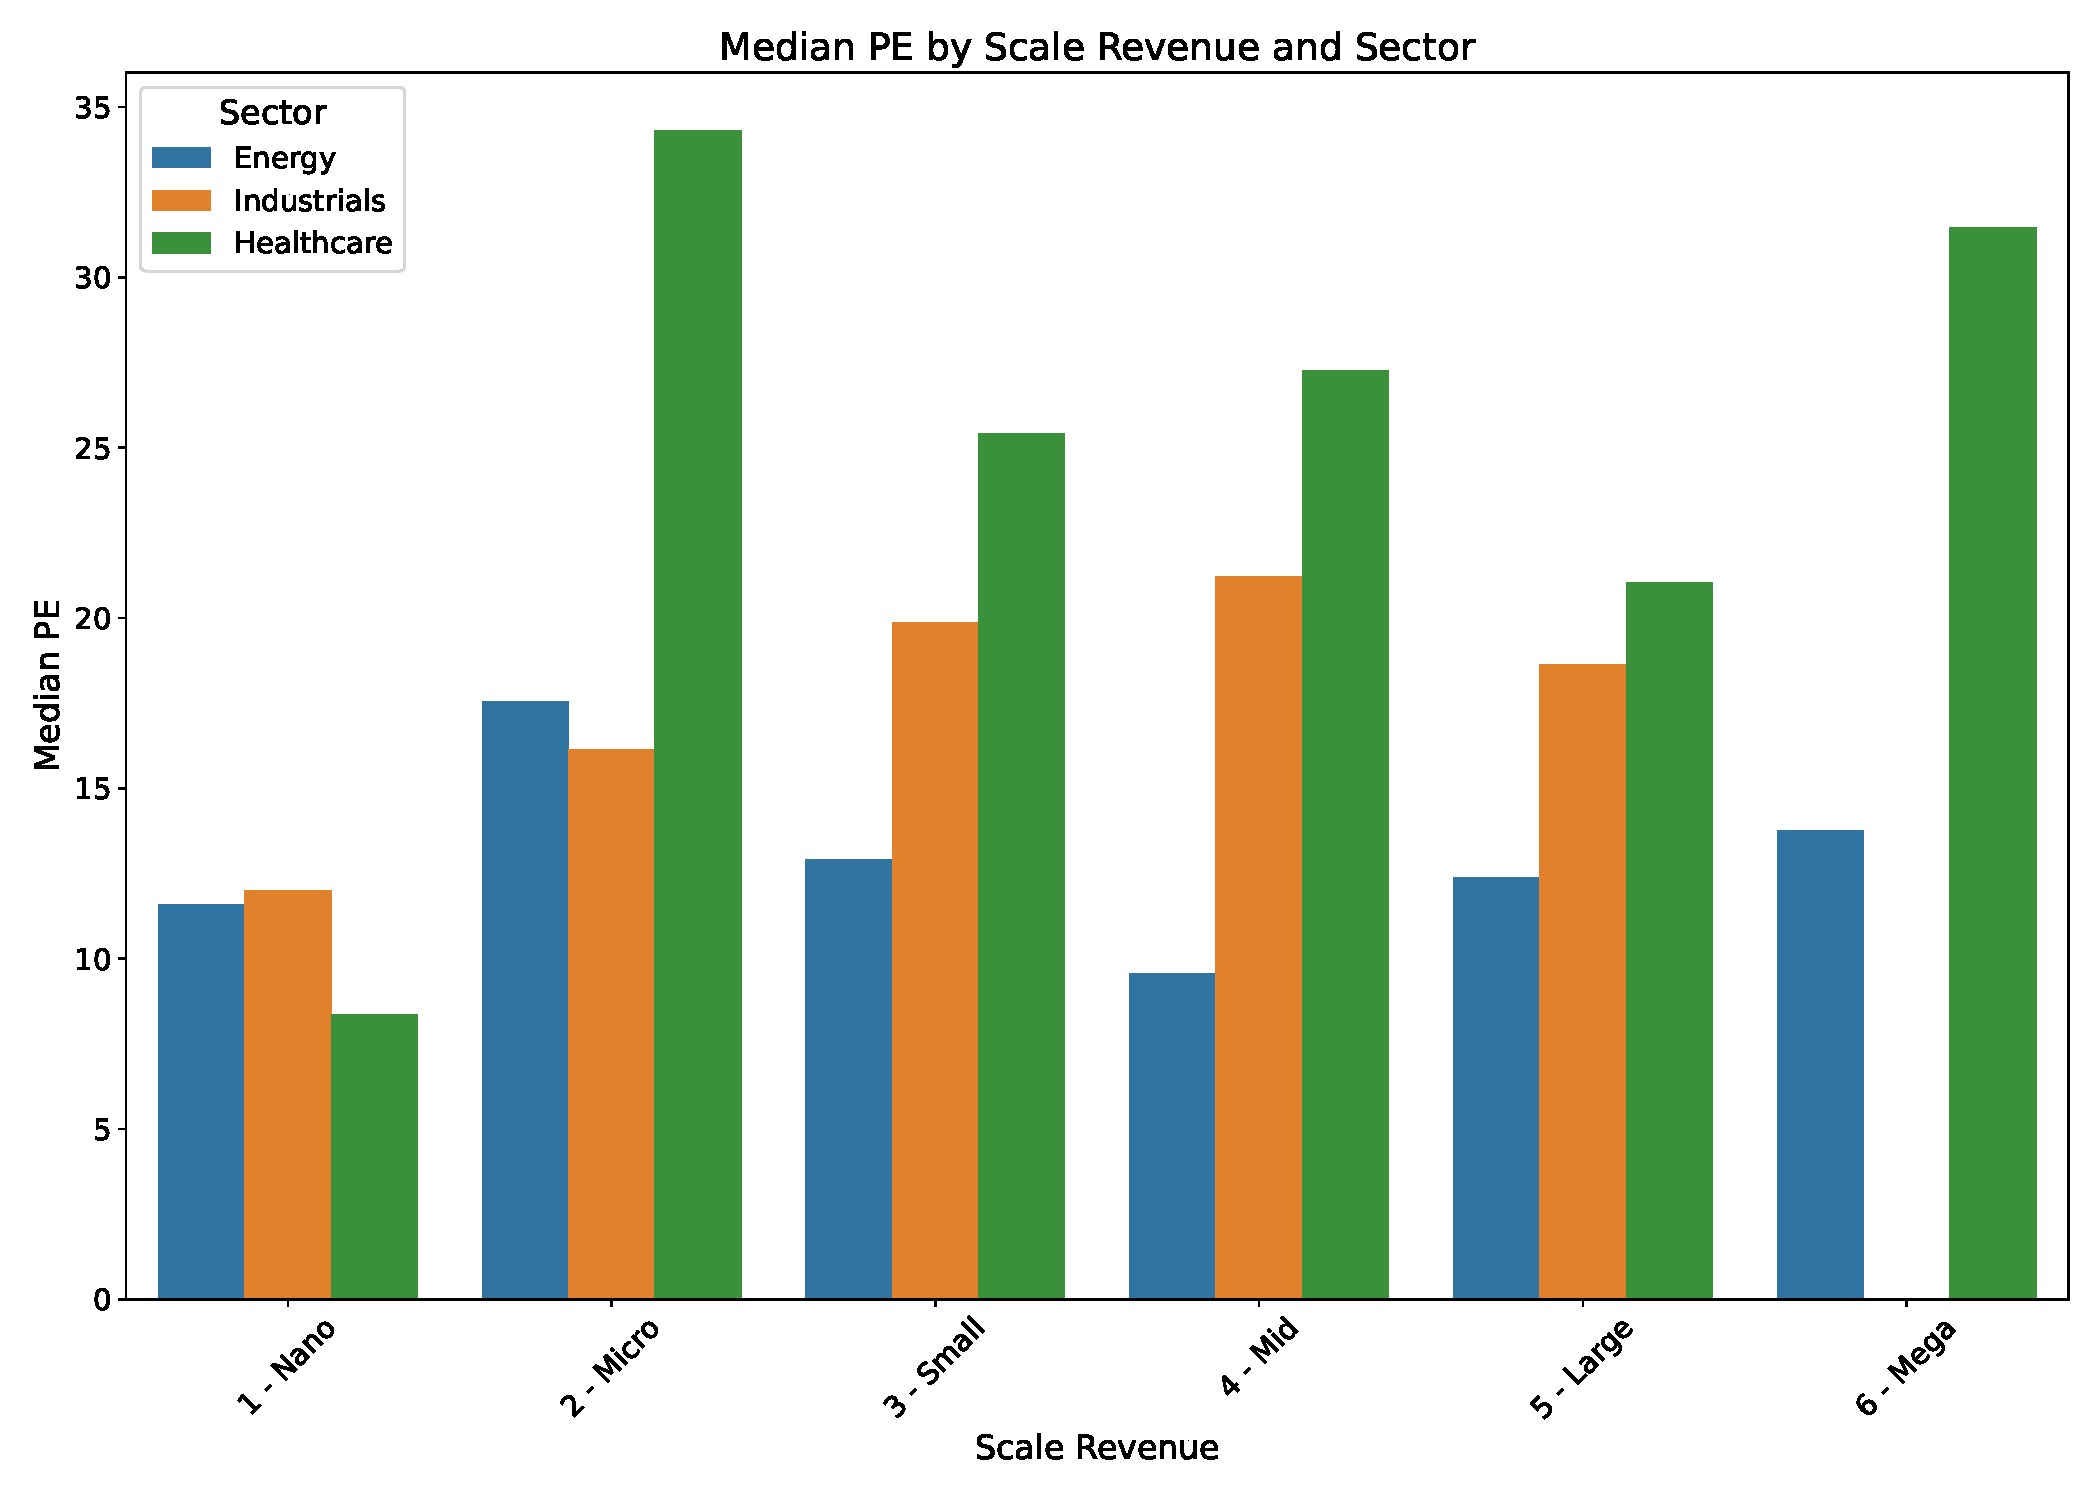
\includegraphics[width=0.9\textwidth]{financial_images/bar_chart_pe_updated.pdf}
  \end{center}
\end{frame} 

\begin{frame}[plain] 
  \begin{center}
  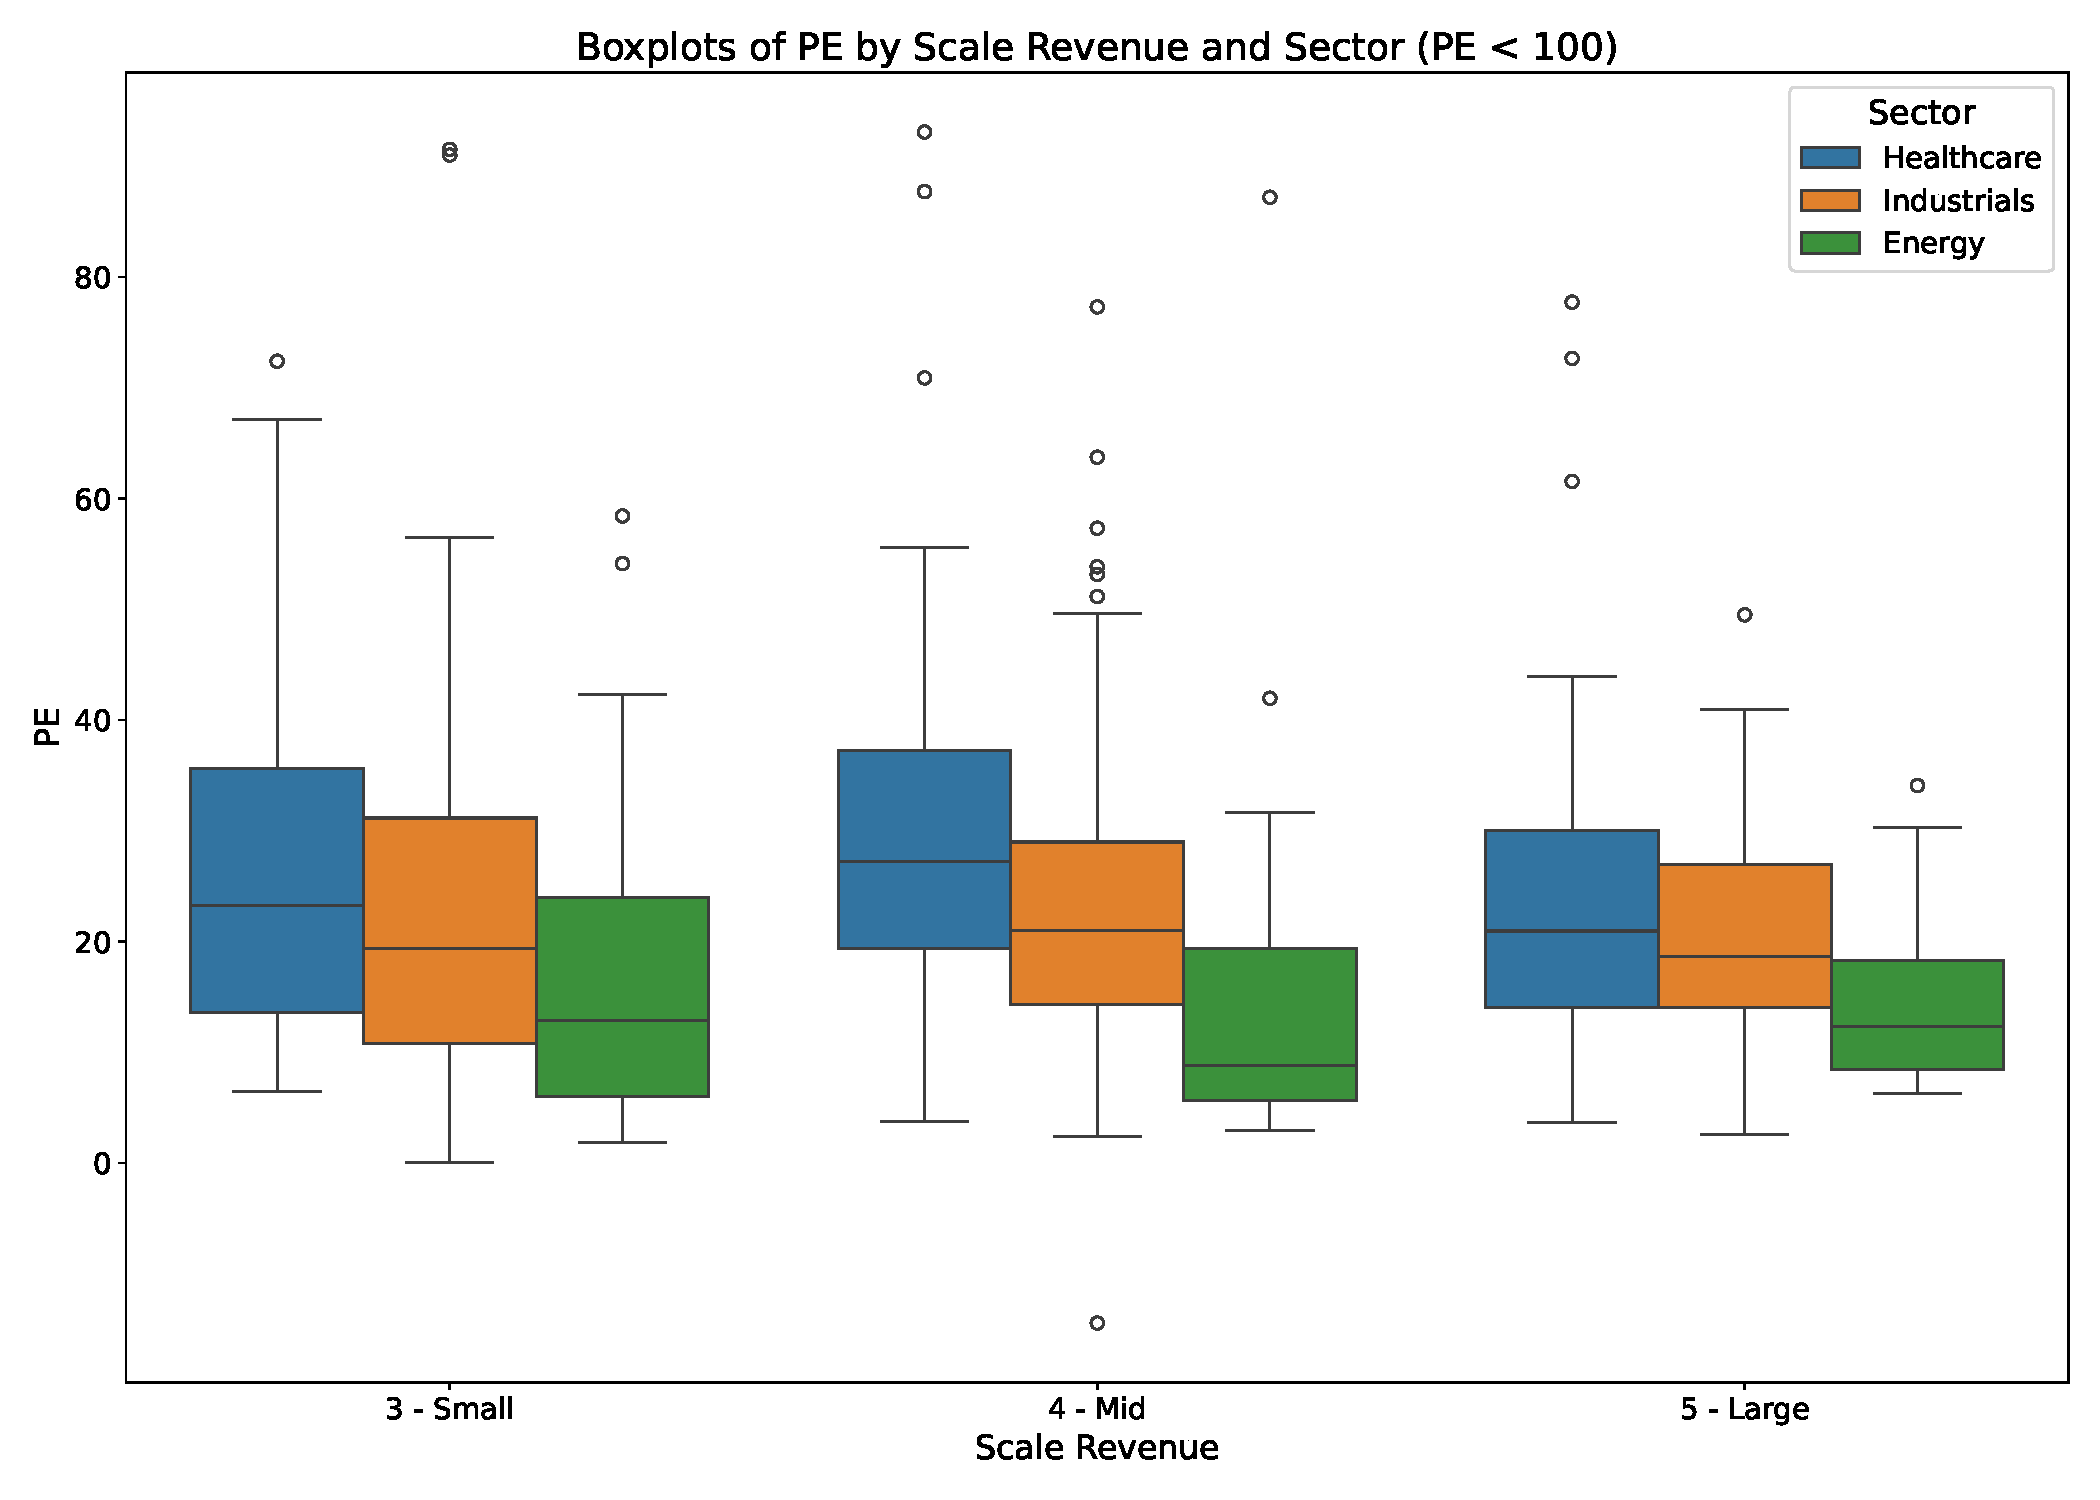
\includegraphics[width=0.9\textwidth]{financial_images/boxplot_pe_updated.pdf}
  \end{center}
\end{frame}

\begin{frame}[plain] 
  \begin{center}
  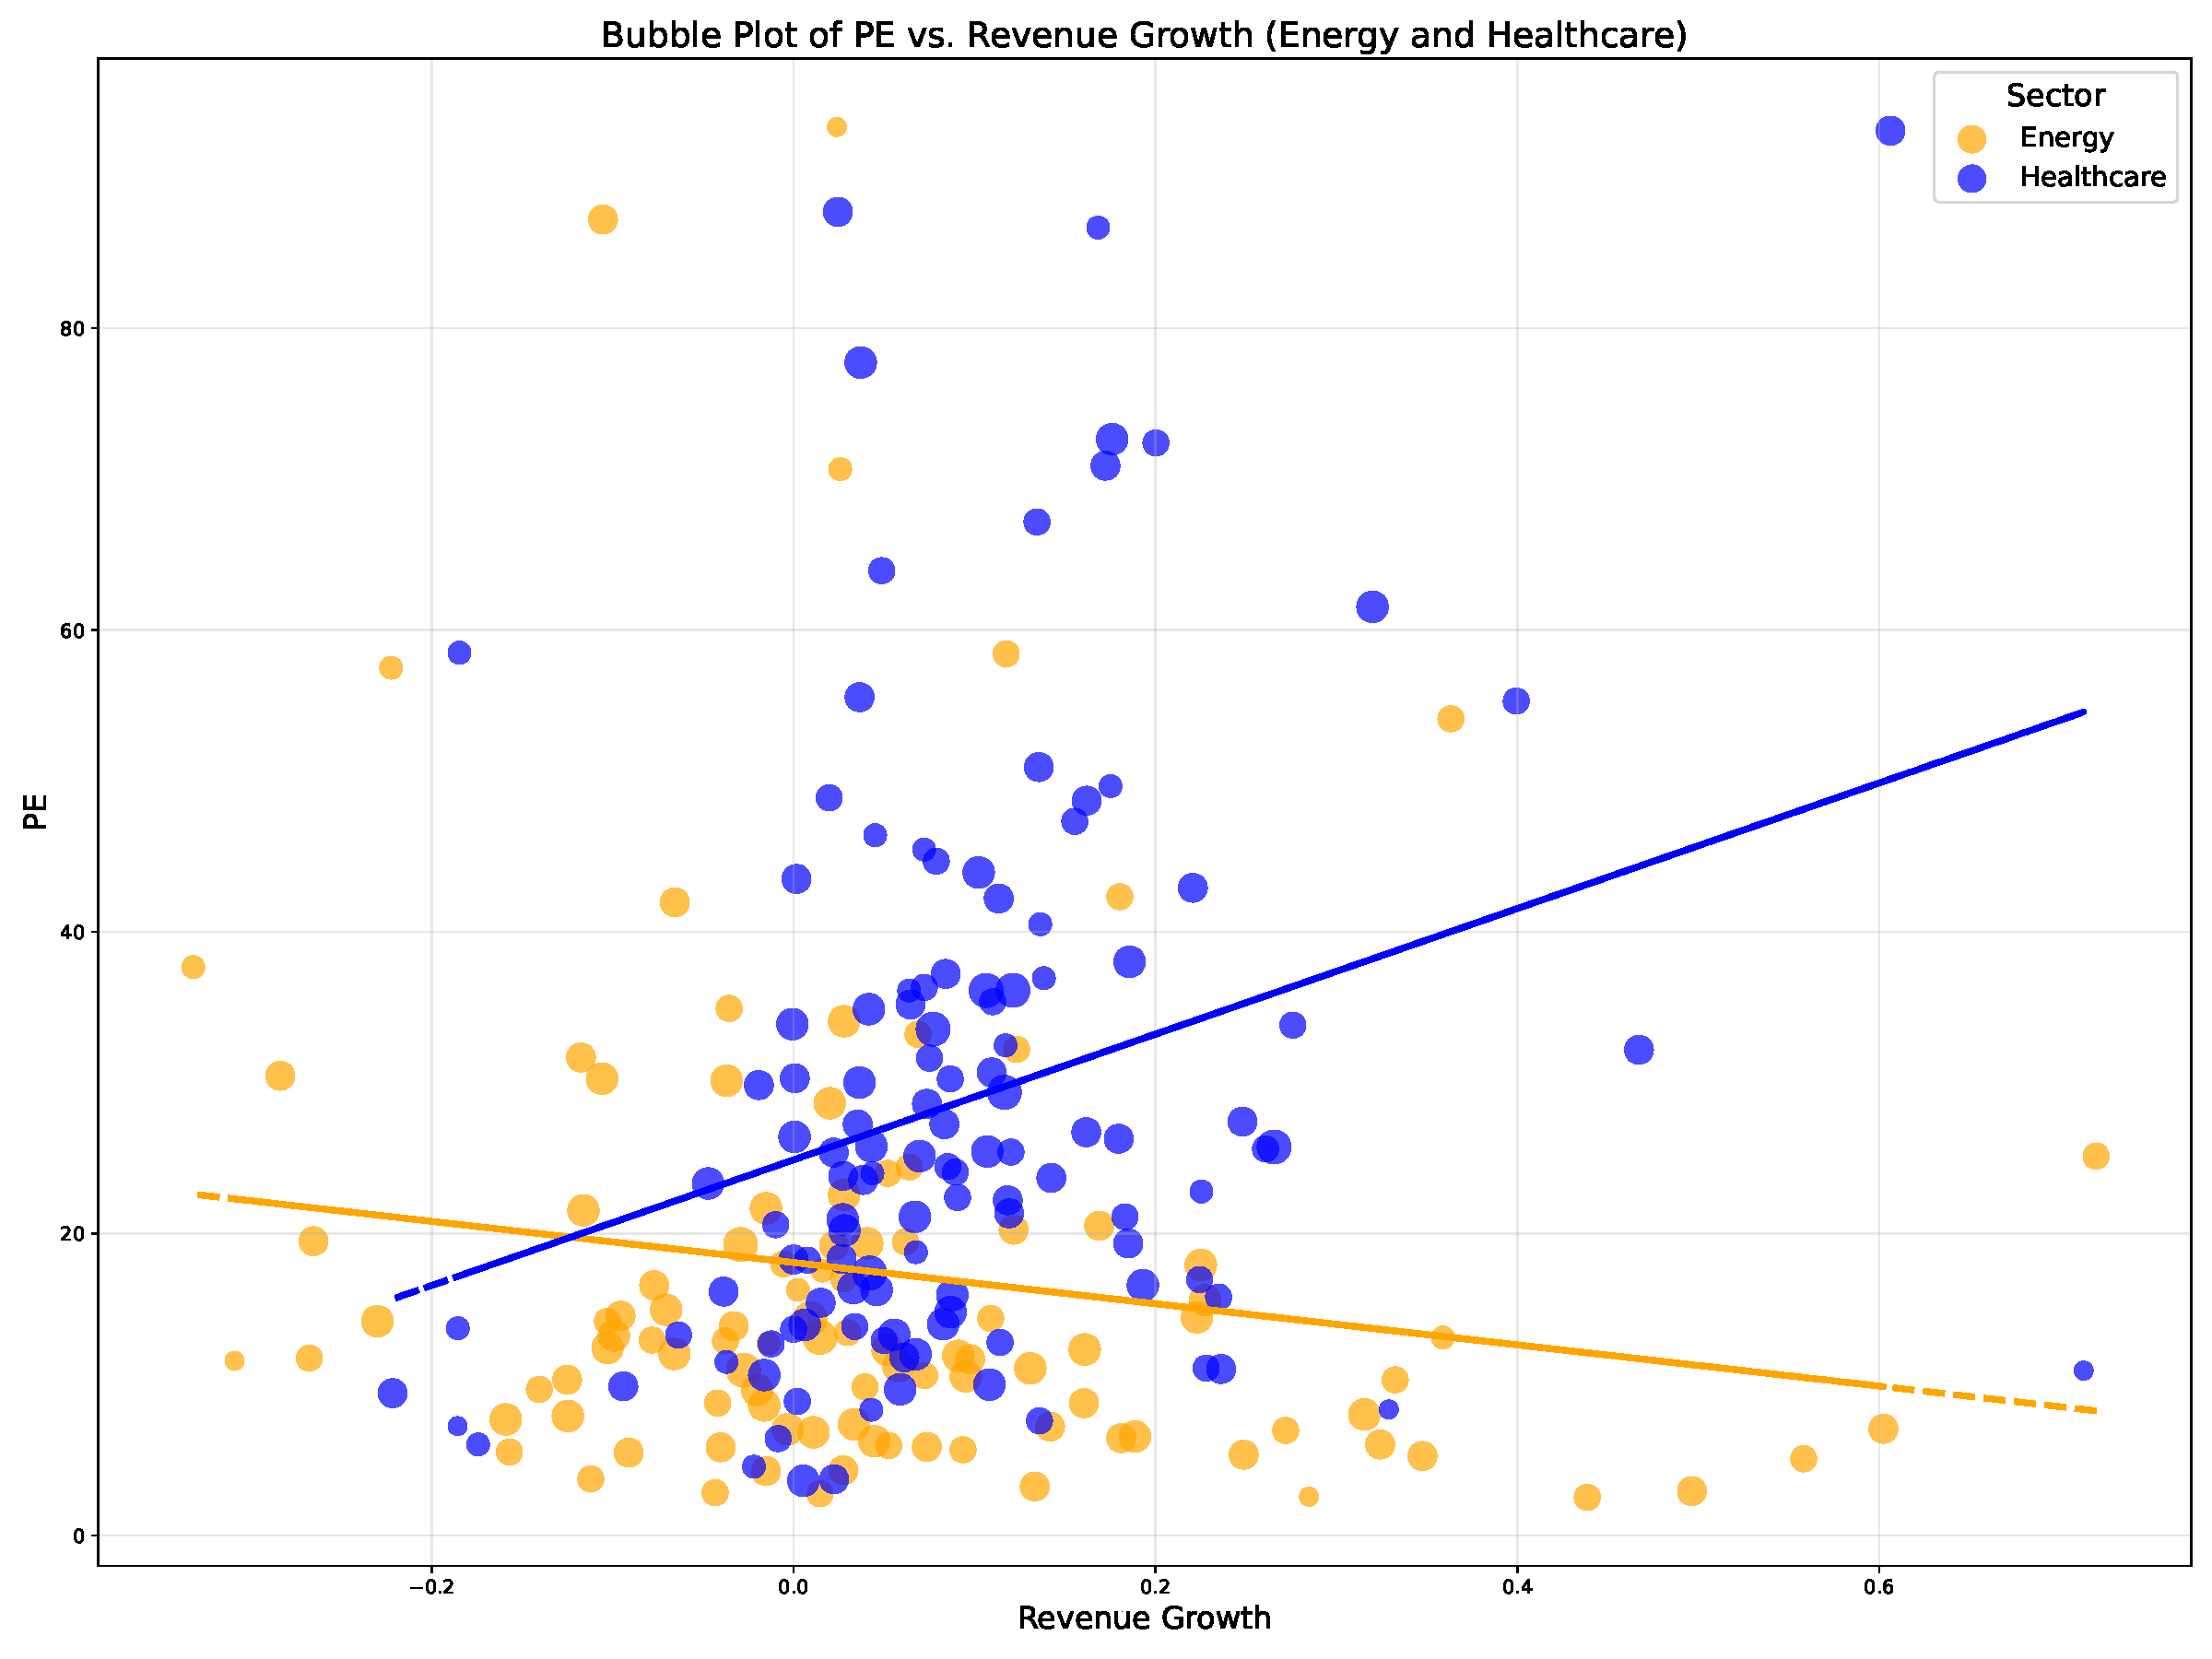
\includegraphics[width=0.9\textwidth]{financial_images/bubble_plot_energy_healthcare.pdf}
  \end{center}
\end{frame}


  \begin{frame}[plain] 
    \begin{center}
    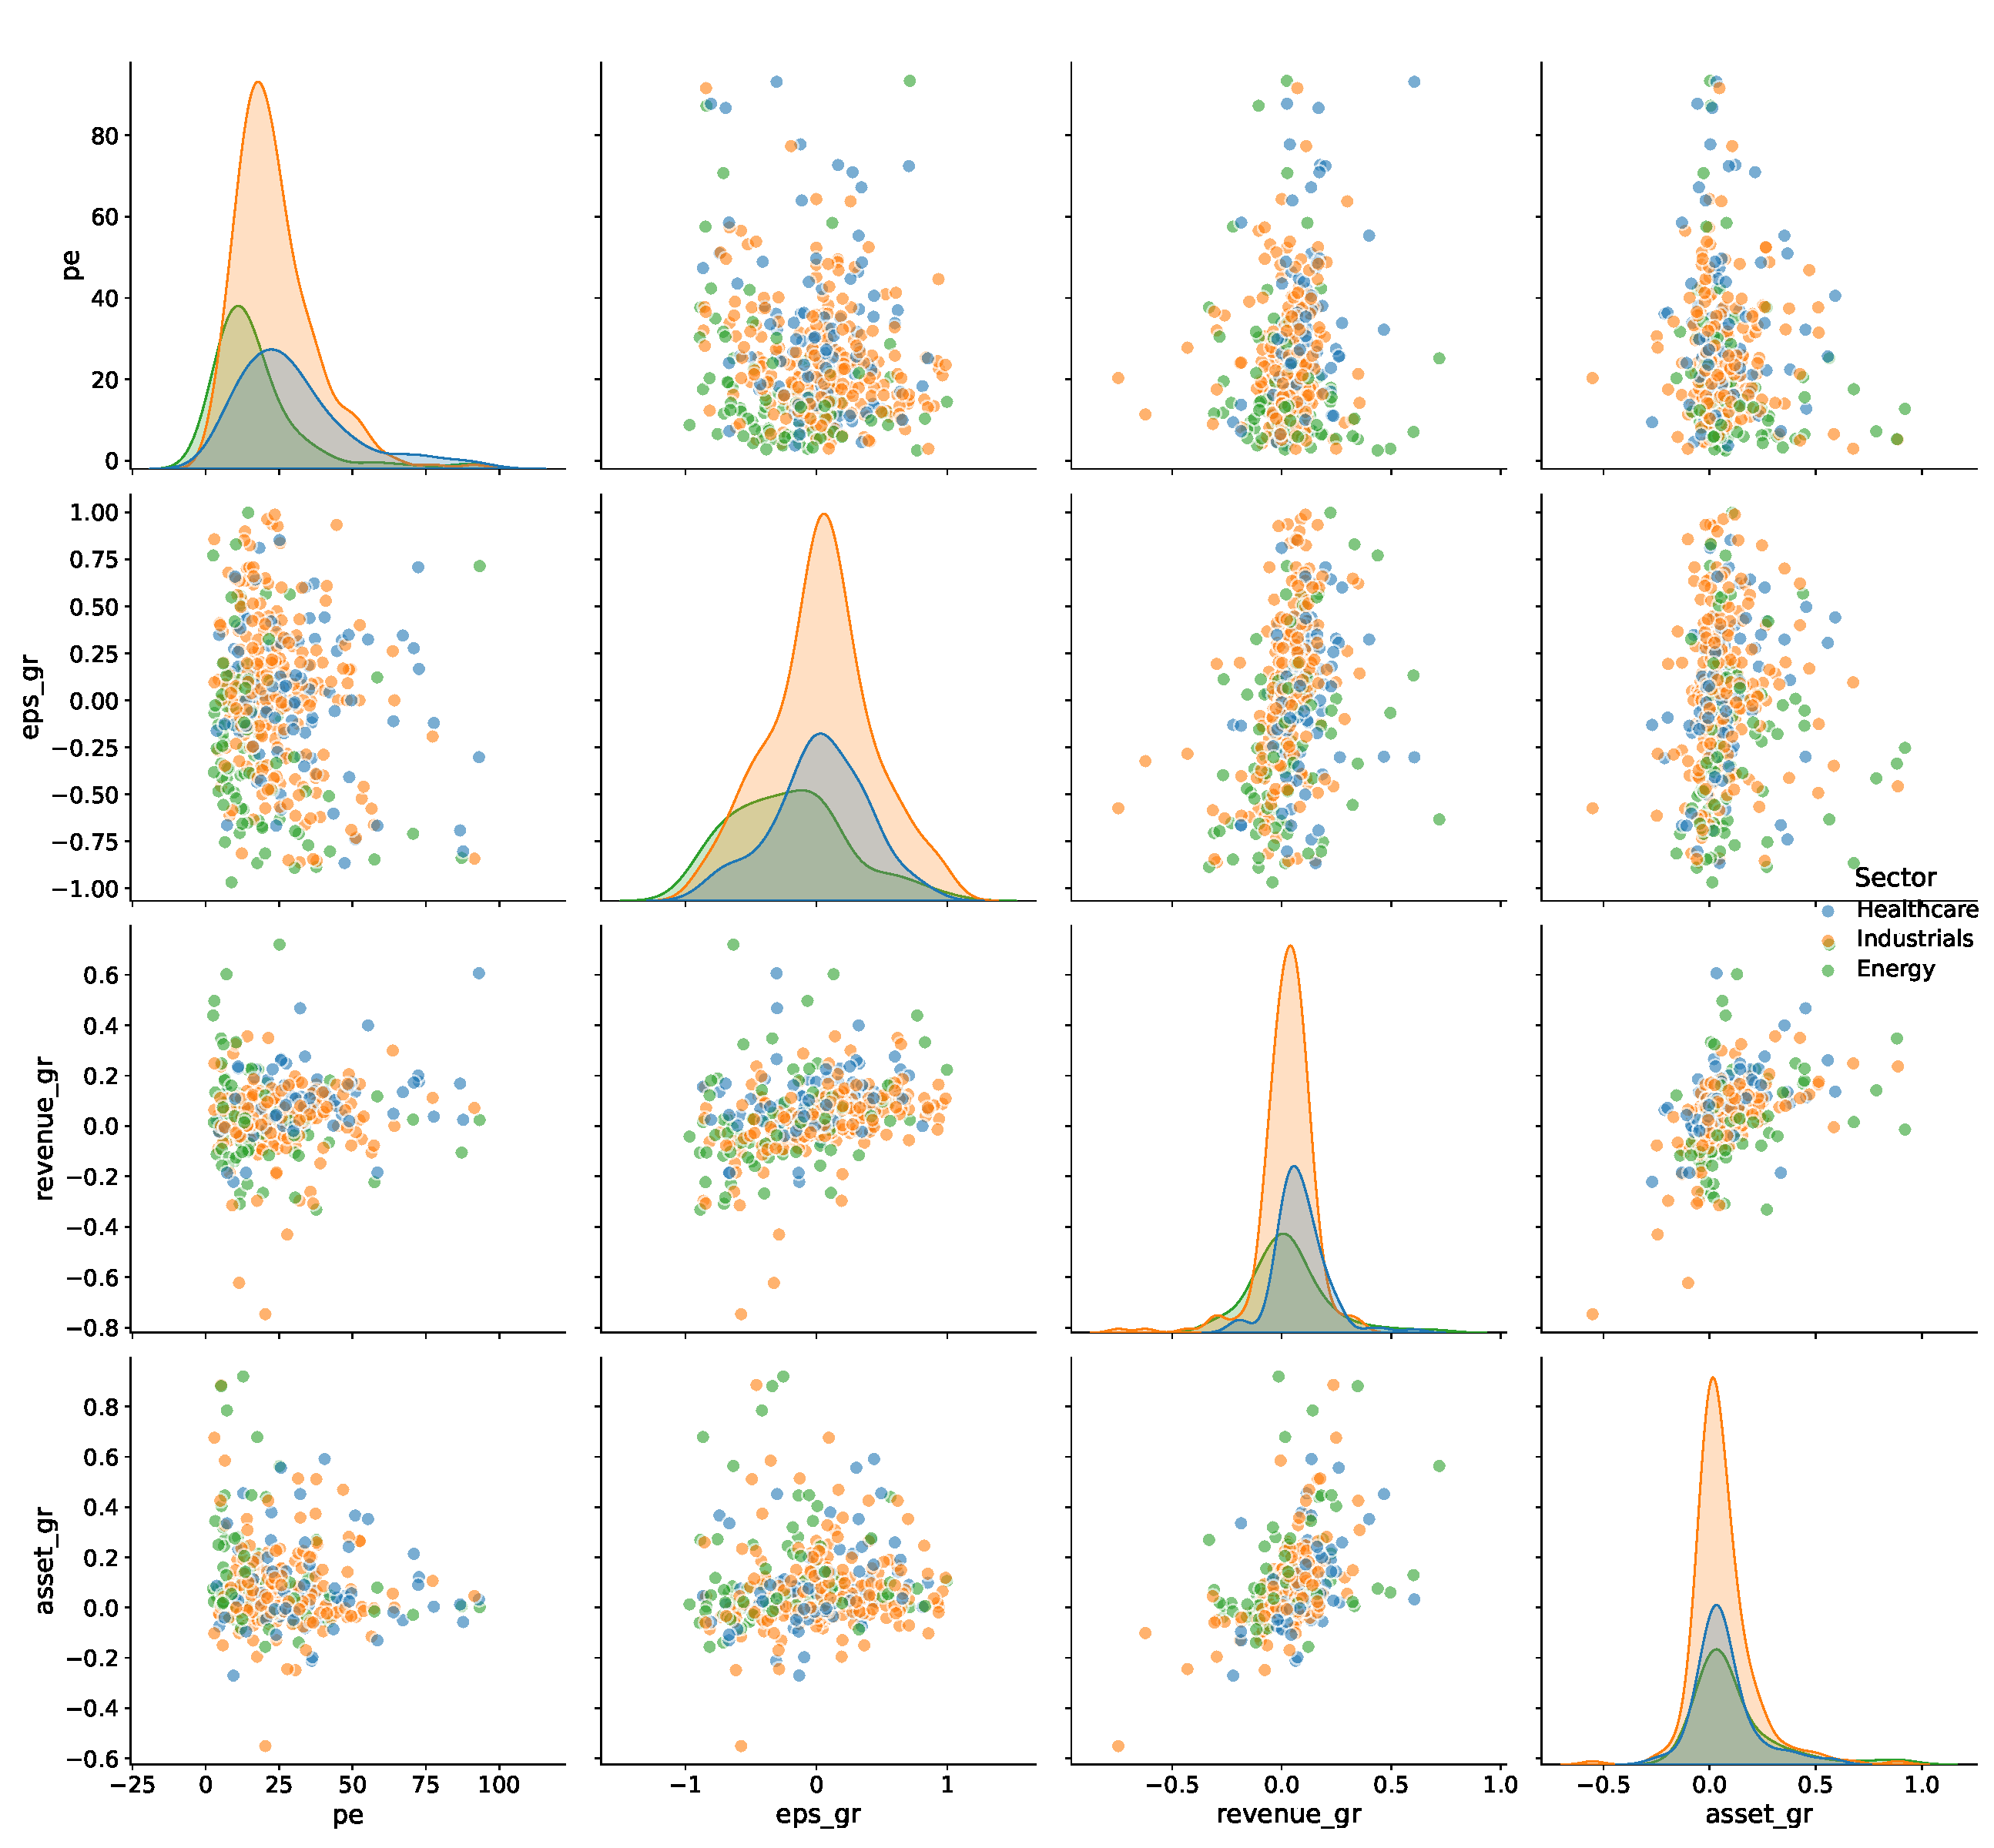
\includegraphics[width=0.9\textwidth]{financial_images/pairplot_metrics_updated.pdf}
    \end{center}
\end{frame}

  \begin{frame}[plain] 
    \begin{center}
    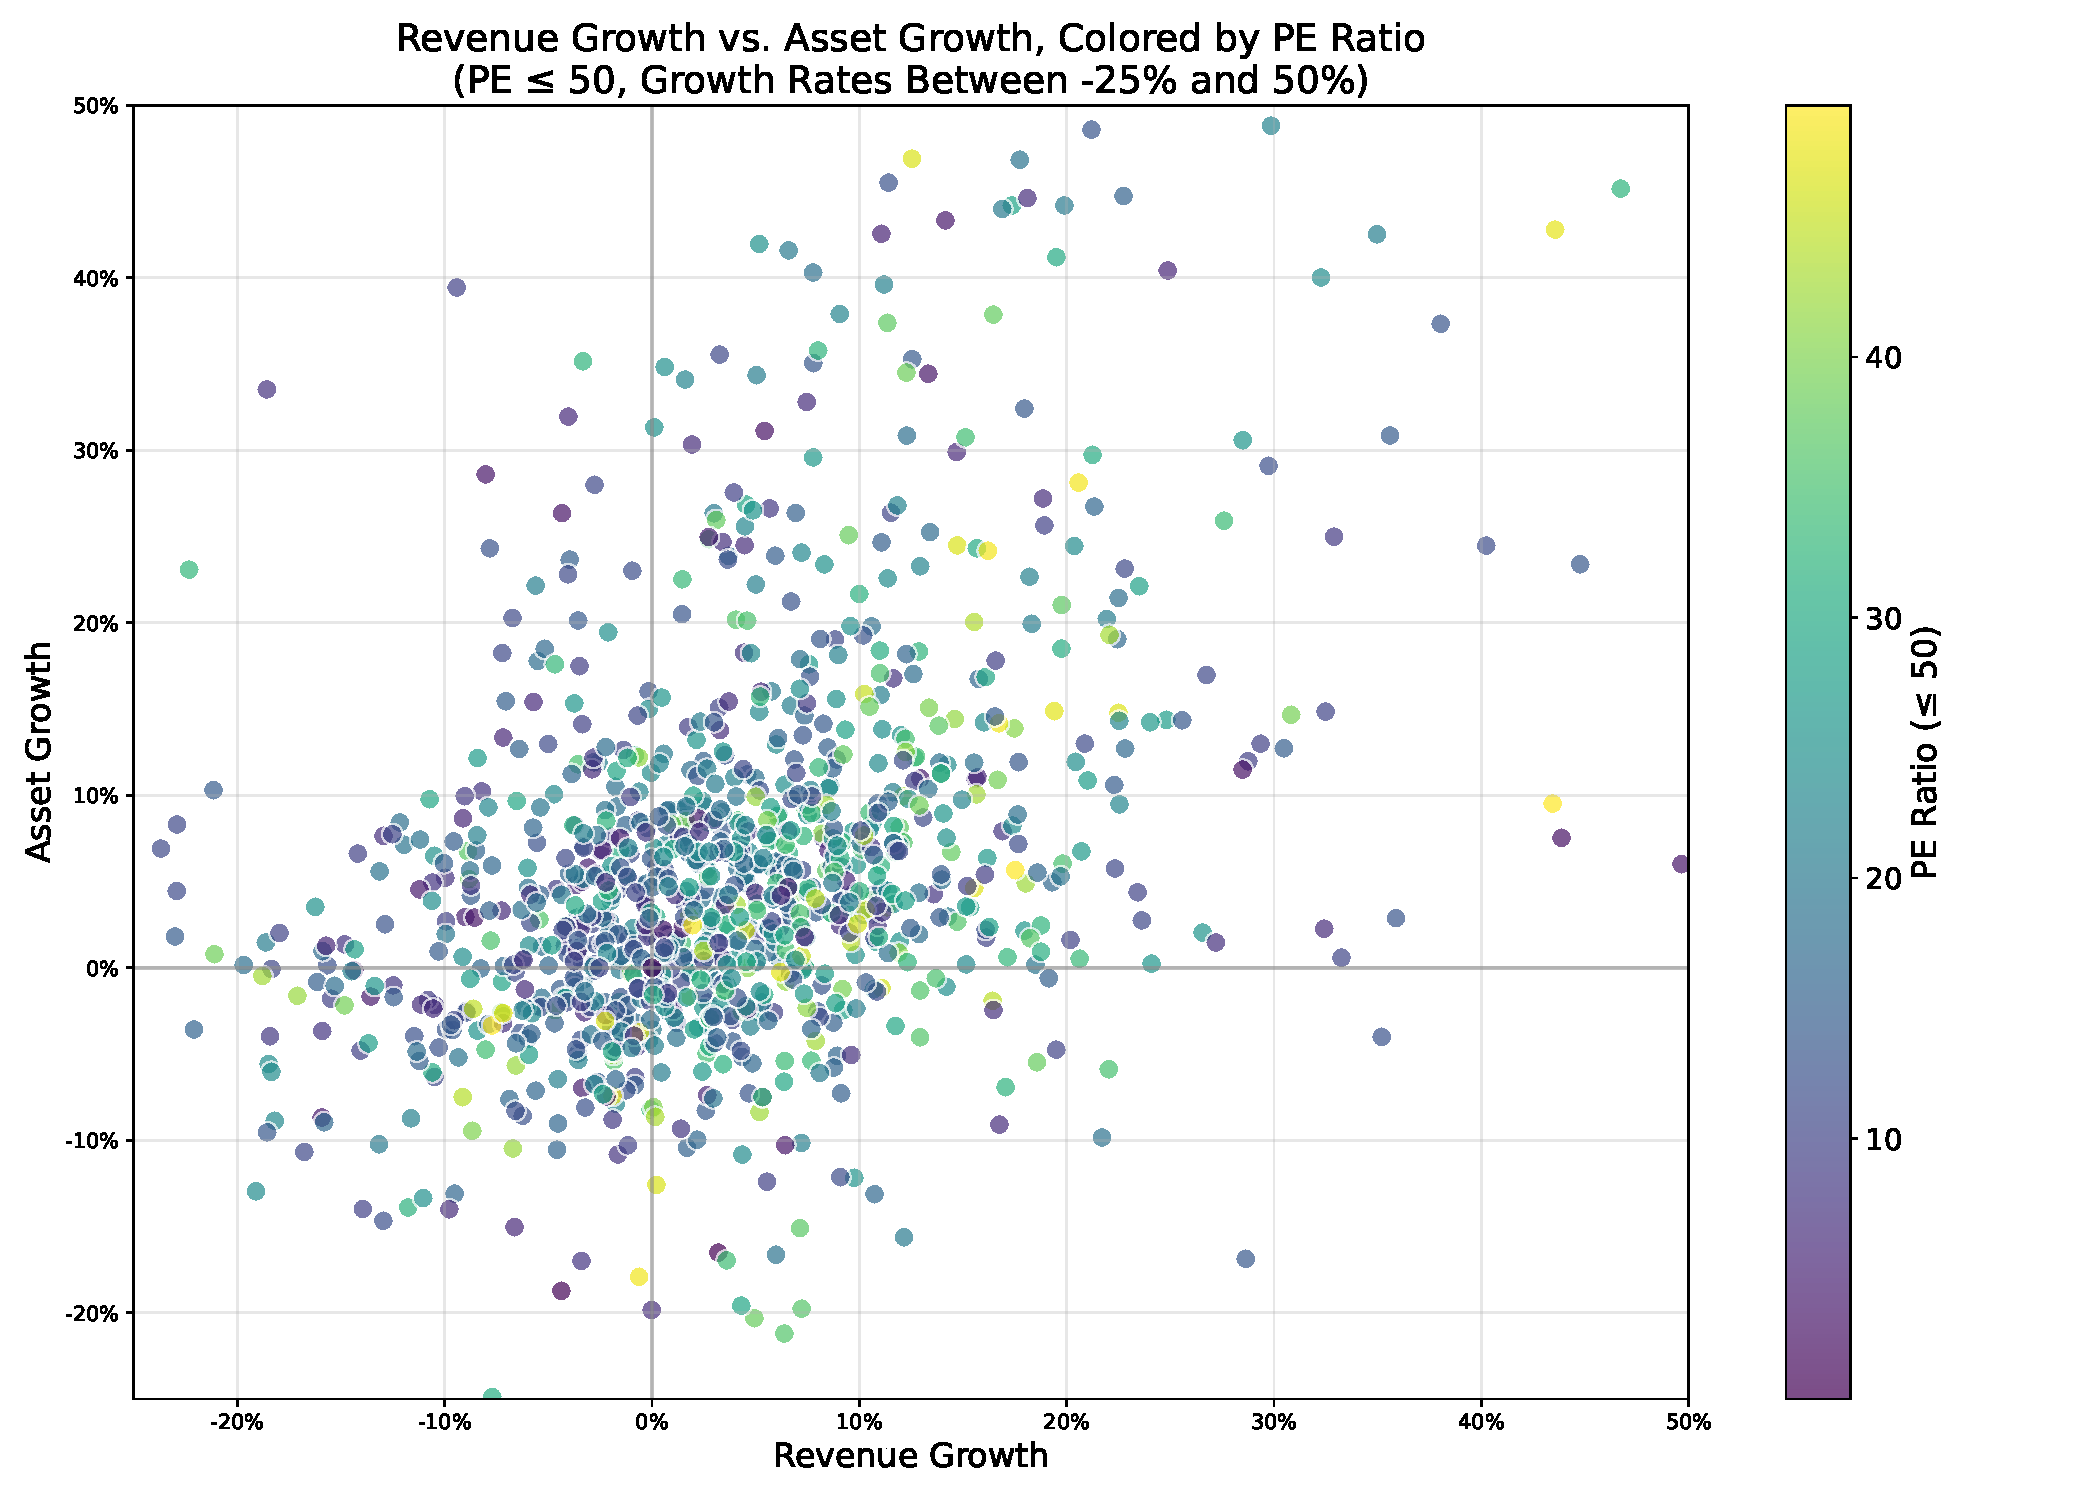
\includegraphics[width=0.9\textwidth]{financial_images/scatter_revenue_asset_pe_restricted.pdf}
    \end{center}
  \end{frame}

  \begin{frame}[plain] 
    \begin{center}
    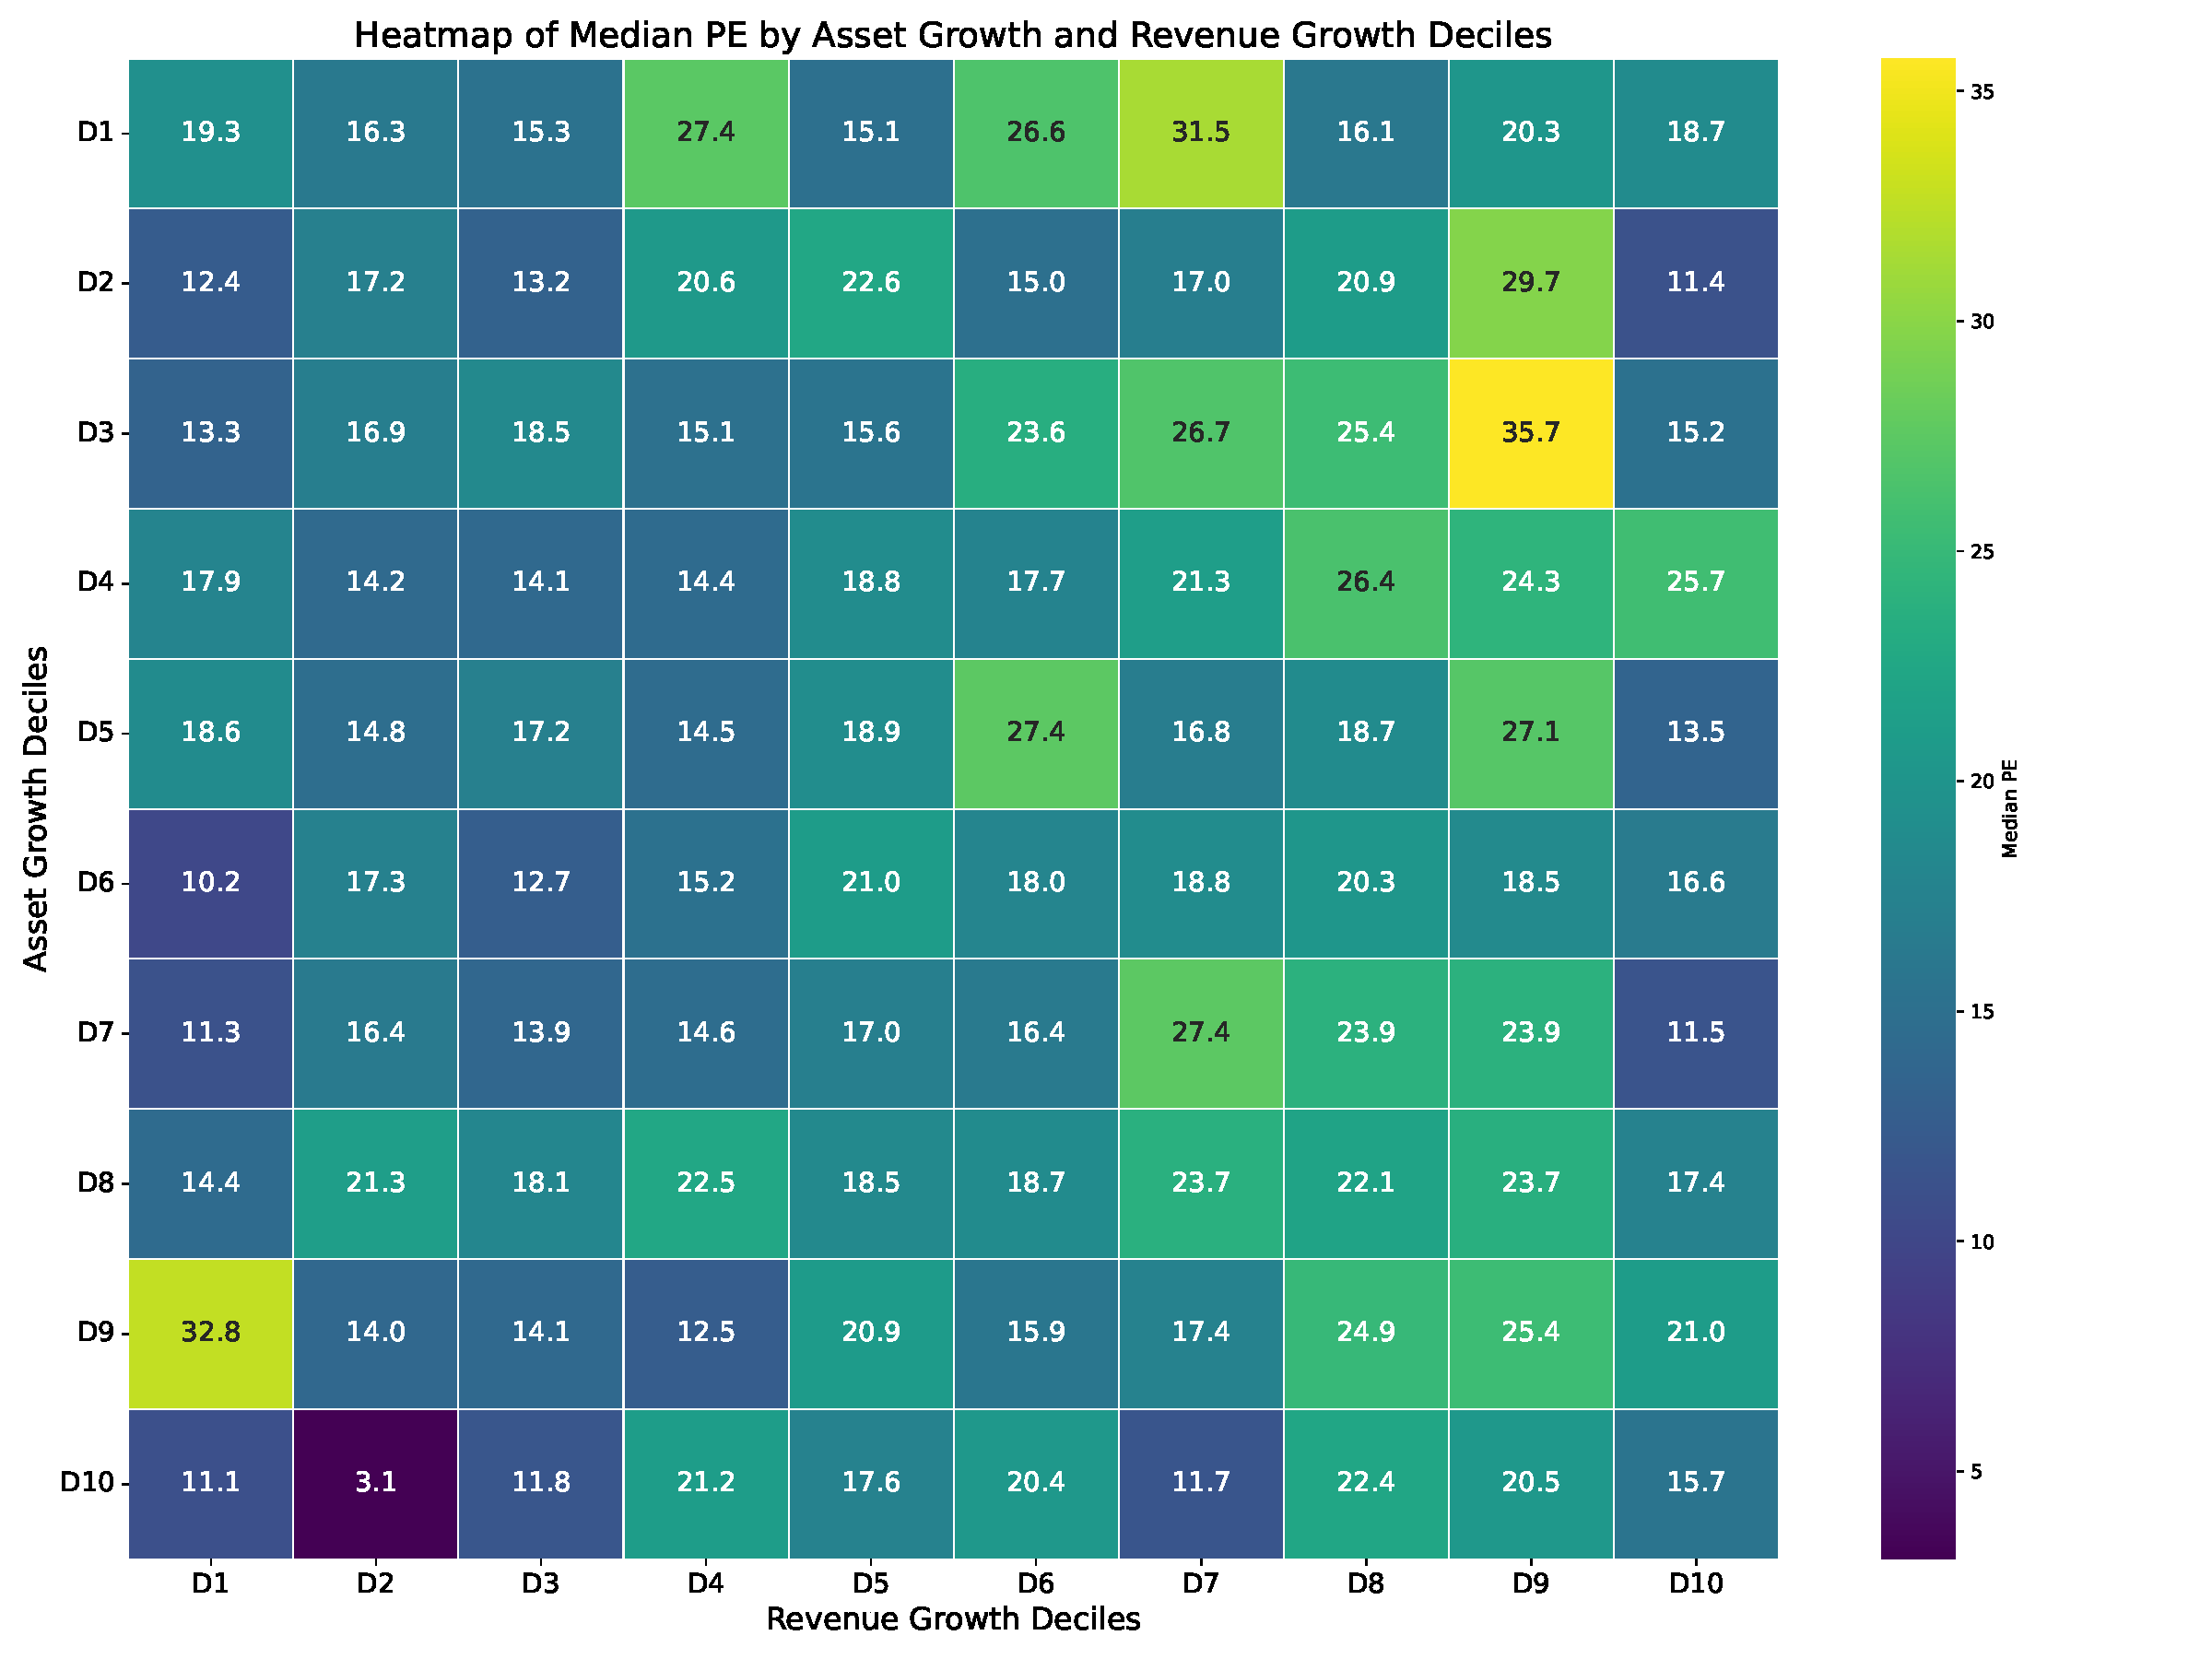
\includegraphics[width=0.9\textwidth]{financial_images/heatmap_pe_by_growth_deciles_viridis.pdf}
    \end{center}
  \end{frame}
  \section{Prompts}

  

\begin{frame}{Example Prompts}
  \begin{itemize}
    \item Create filled density plots of PE by sector in [healthcare, energy].
    \item Create a heatmap of median PE by group with scalerevenue in columns and sector in rows.  Order scalerevenue as nano, micro, small, mid, large, mega.
  \item Filter to sector in [healthcare, industrials, energy].  Create a bar chart of median PE by group with scalerevenue on the x-axis and sector as hue.  
  \item Filter further to scalerevenue in [small, mid, large] and to pe<100.  Create boxplots of PE with scalerevenue on the x-axis and sector as hue.  
  \item Create a bubble plot of PE vs. revenue\_gr with scalerevenue as size and sector as color.  Add a regression line for each sector using the sector color.  
  
  \end{itemize}
\end{frame}

\begin{frame}{More Example Prompts}
  \begin{itemize}
    
  \item Create a pairplot of [pe, eps\_gr, revenue\_gr, asset\_gr] with sector in [healthcare, industrials, energy] as hue.
  \item Create a scatter plot of asset\_gr against revenue\_gr with pe as the color.  Use only observations for which pe<50 and asset\_gr and revenue\_gr are between -25\% and 50\%.
  \item Define categorical variables for deciles of asset\_gr and revenue\_gr.  Create a heatmap of median pe by group with asset\_gr on the y-axis and revenue\_gr on the x-axis.
  \end{itemize}
\end{frame}
\end{document}